%% LyX 2.2.2 created this file.  For more info, see http://www.lyx.org/.
%% Do not edit unless you really know what you are doing.
\documentclass[UTF8]{ctexart}
\usepackage{amsmath}
\usepackage{fontspec}
\usepackage{geometry}
\geometry{verbose,tmargin=2.54cm,bmargin=2.54cm,lmargin=3.18cm,rmargin=3.18cm}
\pagestyle{plain}
\usepackage{graphicx}
\usepackage[unicode=true,pdfusetitle,
 bookmarks=true,bookmarksnumbered=true,bookmarksopen=true,bookmarksopenlevel=1,
 breaklinks=false,pdfborder={0 0 1},backref=false,colorlinks=false]
 {hyperref}

\makeatletter

%%%%%%%%%%%%%%%%%%%%%%%%%%%%%% LyX specific LaTeX commands.
%% Because html converters don't know tabularnewline
\providecommand{\tabularnewline}{\\}

%%%%%%%%%%%%%%%%%%%%%%%%%%%%%% User specified LaTeX commands.
% 如果没有这一句命令,XeTeX会出错,原因参见
% http://bbs.ctex.org/viewthread.php?tid=60547
\DeclareRobustCommand\nobreakspace{\leavevmode\nobreak\ }

\makeatother

\usepackage{listings}
\lstset{language={C++},
basicstyle={\linespread{1} \ttfamily },
frame=single,
keywordstyle={\bfseries},
tabsize=4,
breaklines={true}}
\usepackage{xunicode}
\renewcommand{\lstlistingname}{列表}

\begin{document}

\title{基于时空数据分析的决策支持 实验报告}

\author{卢力韬 15307130084@fudan.edu.cn}
\maketitle

\section{环境}

Ubuntu 16.04.1 + Clion 

编译命令: 

g++ -std=c++11 Topic\_A.cpp -o Topic\_A -O2

g++ -std=c++11 Topic\_B.cpp -o Topic\_B -O2

(g++ 5.4.0)

\section{数据结构与算法}

\subsection{出租车基础分析}

本部分要求通过出租车的轨迹计算出每个司机每天的收入,以及司机收入在时间上的分布情况。但是读入文件是一件十分麻烦的事情,为了方便我们之后的程序,在这里可以先定义一个类CSVrow,并重载它的读入函数。

\begin{lstlisting}
class CSVrow : public vector<string> {
    friend istream &operator>>(istream &str, CSVrow &data);
private:
    void get_row(istream &src) {
        string buf, ele;
        getline(src, buf);
        if (!buf.empty()) buf.pop_back();
        stringstream s_in(buf);

        while (getline(s_in, ele, ','))
            push_back(ele);
    }
};
istream &operator>>(istream& str, CSVrow &data) {
    data.clear();
    data.get_row(str);
    return str;
}
\end{lstlisting}

这样只用简单的一句\texttt{fin >\textcompwordmark{}> r}; 就可以读入一整行的内容了,十分方便。

读入了数据之后,我们可以开始计算。但是经过实验发现轨迹数据有十分多的错误。比如:在零点时到底是否为空车;空车与非空车状态会无意义的切换导致可能将距离很小的也当成订单计入司机收入;还有轨迹产生漂移,导致瞬时速度极大。这些在计算收入的时候都需要考虑。我在计算的时候,根据轨迹文件的注释一栏,Takein,Takeout来查看是否为空车。默认零点开始为空车。并且把距离大于0.01km的订单计入司机收入。

\subsection{消极策略}

本部分要求模拟司机接单过程,如果3km内有订单,则以最高速驶向次订单,并载客。载客完毕之后一直在原地等待,直到3km内又出现订单为止。

实现本部分,我们要先读入路网。

这里,我做了一个优化,在建图的时候,对于一条路中间度数为二的点,我们可以不加到图里。而只将每条路的头与尾当成这个图的节点。这样可以大大减少图中点的数量(减少80\%)。

要模拟这部分,我们要实现:
\begin{enumerate}
\item 算出一个点在路网上的投影
\item 查询任意一个点3km内是否有订单
\item 算出路网上任意两点的最短路
\item 查询3km内路网距离最近的点
\end{enumerate}

\subsubsection{算出一个点在路网上的投影}

我们用插入分点的方法来计算投影。即对于一条路,如果它两个相邻的轨迹点的距离大于50米,那么我们就在这两个点中间插入若干个点,使得相邻两个点的距离都小于50m。这样,我们查询任意一个点在路网上的投影,就相当于查询路网上所有点与我们插入的分点中距离查询点最近的是什么。

可以知道,这样得到的最近点距离真实的投影误差不会超过50m。考虑到路网输入的经纬度座标也仅仅只有6位有效数字,这样的误差是可以接受的。

接下来我们用网格索引来实现,查询最近点的功能。网格索引,即\texttt{vector<Point> blk{[}XNUM{]}{[}YNUM{]};}

对于每个点,我们可以通过\texttt{int ix = (p.longitude - min\_x) / intv\_x, iy
= (p.latitude - min\_y) / intv\_y;}来知道它是属于$(ix,iy)$这个网格的。每次插入或删除一个点,只需要在它对应的那个网格里面进行操作即可。

在网格索引中寻找最近点:我们只用暴力的看$(ix,iy)$这个网格与其周围的8个网格内的所有点,找出距离最小的即可。将网格的长、宽调至一个适宜的值之后,经过实验,每次查询最近点只需要调用30\textasciitilde{}80次dist(计算两点距离)函数。这样的复杂度是可以接受的。考虑到常数问题,这甚至比K-d
tree更优。

\subsubsection{查询任意一个点3km内是否有订单}

同样的用网格索引的方法。

维护一个网格索引,内含当前时间之前的所有订单。注意,请与上一节中的网格索引做区分,它们含的点是不同的。而且因为这个网格索引内的点比较稀疏,经过实验,我们的网格长宽均为前者的15倍较好。

查询3km内点的方法和前面也类似。我们看查询点3km内覆盖到了哪些网格, 暴力的看这些网格内部的点哪些是3km内的。

\subsubsection{算出路网上任意两点的最短路}

这里用了A{*}算法。与Dijkstra算法不同,A{*}算法在令元素入有限队列的时候用的是启发函数,这样在真实最短路上的点很有可能先入队。用时比Dijkstra更短一些。经过测试,A{*}与Dijkstra的对比如下:

\begin{table}[h]
\begin{centering}
\begin{tabular}{|c|c|c|c|}
\hline 
邯郸-张江 & 邯郸-人民广场 & 二附中-人民广场 & 张江-长泰\tabularnewline
\hline 
\hline 
1987 & 1083 & 4217 & 63\tabularnewline
\hline 
26671 & 7594 & 18706 & 693\tabularnewline
\hline 
\end{tabular}
\par\end{centering}
\caption{A{*}与Dijkstra入队的节点数对比}
\end{table}

可以看到,A{*}在长、短距离的求解上都比Dijkstra算法要优。

\subsubsection{查询3km内路网距离最近的点}

本来我们获得了3km内所有的点之后,就可以用上一节的A{*}算法求出所有点的路网距离,取最小就可。但是实践中发现有时3km内点会多达几千个。于是考虑在3km内点多余500个时候,直接用Dijkstra算法一次性求出所有点的路网距离,而不是用A{*}一个个的求。应用这个优化之后,程序用时有9.7\%的提升。

\subsection{积极策略}

本部分与消极策略仅仅不同与:当没有订单时,司机以10km/h低速漫游,直到遇到订单为止。

我们需要一个新的操作:随机漫游。

为此实现了一个函数:\texttt{queue<Point> gen\_random\_path(Point \&p)}.返回一个随机的轨迹。具体为随机走10条近期没走过的路。将路上的所有点都加入轨迹中,并返回之。

此外,这部分还有一个优化:在随机漫游时,我们需要不停地查看3km内是否有订单。我们知道,这次查询的点与上次查询的点相距很近(因为都在低速随机漫游的轨迹上)。这样3km内的大多数点都是不变的,我们可以只看有变化的新覆盖到的网格,与新没覆盖到网格的变化。(如图\ref{fig:=007F51=00683C=007D22=005F15=0067E5=008BE23km=005185=007684=004F18=005316})

\begin{figure}[h]
\begin{centering}
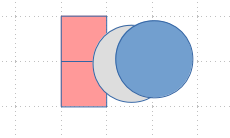
\includegraphics{pasted1}
\par\end{centering}
\caption{网格索引查询3km内的优化,圆心代表3km的范围;红色为改变的网格\label{fig:=007F51=00683C=007D22=005F15=0067E5=008BE23km=005185=007684=004F18=005316}}

\end{figure}


\subsection{TopicA的补充说明}

在计算消极策略与积极策略时,我发现消极策略与积极策略的结果并无大不同。这是因为生成订单过多,根本不会出现3km内没有订单的情况,司机没有间隔的不停接单。为了模拟更有意义,将订单随机减少了20倍,并且加了一个限制:如果订单等待超过15分钟,乘客会自动取消订单。这样两种策略就有显著差别了。

\subsection{POI推荐}

这部分可以通过前面司机的路径数据来推测餐馆的热门程度。定义餐馆的积分函数$score$,每个下车点对$score$的贡献为一个分段函数$f(dis)$
($dis$为下车点与餐馆的路网距离) 
\[
f(dis)=\begin{cases}
10 & dis<10m\\
7 & dis\in(0,1,1]km\\
6 & dis\in(1,2]km\\
3 & dis\in(2,3]km
\end{cases}
\]

每次查询某个点附近的餐馆,先用网格索引查询3km的餐馆,再根据$score\times k$排序,其中$k$是一个随路网距离增大而减小的系数。

此外,实验发现,推荐出来的餐馆有时会有聚团现象。为此,加了一个判断:如果前10个推荐的最大距离小于1km,则再推荐5个远离前十个的餐馆。

\section{实验结论}

\subsection{基础分析}

司机一天收入的分布情况如图\ref{fig:=0053F8=00673A=004E00=005929=006536=005165=005206=005E03}所示,司机每日平均收入为671.67元,考虑到司机还有租金等成本,这个收入还是合理的。

\begin{figure}[h]
\includegraphics{\string"/home/lulitao/文档/Data Structure Homework/Final Project/graphs/dir_distro\string".pdf}\caption{司机一天收入分布\label{fig:=0053F8=00673A=004E00=005929=006536=005165=005206=005E03}}

\end{figure}

分时段的分布如图\ref{fig:=0053F8=00673A=006536=005165=005206=0065F6=006BB5=005206=005E03}所示

\begin{figure}[h]
\includegraphics{\string"/home/lulitao/文档/Data Structure Homework/Final Project/graphs/time_distro\string".pdf}

\caption{司机收入分时段分布\label{fig:=0053F8=00673A=006536=005165=005206=0065F6=006BB5=005206=005E03}}

\end{figure}

可以看到,在午夜3\textasciitilde{}6点出现了一个收入的低谷,这也与我们的日常生活经验相符。

\subsection{消极策略}

消极策略司机24小时平均收入为1221元。司机的收入分布如图\ref{fig:=006D88=006781=007B56=007565=004E0B=0053F8=00673A=006536=005165=005206=005E03}所示。可以看到,大部分司机集中在2200\textasciitilde{}2700这个区段。但也有一部分司机收入小于500。这可能是因为消极策略下收入与起始点有很大关系。如果起始点处于偏远的位置,司机就要在原地等待很久。

\begin{figure}[h]
\includegraphics{\string"/home/lulitao/文档/Data Structure Homework/Final Project/graphs/neg_d\string".pdf}

\caption{消极策略下司机收入分布\label{fig:=006D88=006781=007B56=007565=004E0B=0053F8=00673A=006536=005165=005206=005E03}}
\end{figure}

各个时间段所有司机总收入如图\ref{fig:=006240=006709=0053F8=00673A=00603B=006536=005165=0065F6=0095F4=005206=005E03}所示。可以看到,临近午夜时,司机的总收入有大幅下降。这是订单在午夜变得更少,原地等待更难接到单之故。

\begin{figure}[h]
\includegraphics{\string"/home/lulitao/文档/Data Structure Homework/Final Project/graphs/neg_t\string".pdf}

\caption{消极策略下所有司机总收入时间分布\label{fig:=006240=006709=0053F8=00673A=00603B=006536=005165=0065F6=0095F4=005206=005E03}}

\end{figure}


\subsection{积极策略}

积极策略所有司机24小时平均收入1437元。司机的收入分布如图\ref{fig:=0079EF=006781=007B56=007565=004E0B=0053F8=00673A=006536=005165=005206=005E03}所示。可以看到,比起消极策略,低收入的司机变少了很多。可见低速巡游确实可提升收入。

\begin{figure}[h]
\includegraphics{\string"/home/lulitao/文档/Data Structure Homework/Final Project/graphs/pos_d\string".pdf}

\caption{积极策略下司机收入分布\label{fig:=0079EF=006781=007B56=007565=004E0B=0053F8=00673A=006536=005165=005206=005E03}}
\end{figure}

各个时间段所有司机总收入如图\ref{fig:=0079EF=006781=007B56=007565=004E0B=006240=006709=0053F8=00673A=00603B=006536=005165=0065F6=0095F4=005206=005E03}所示。可以看到,积极策略下,收入沿时间分布反倒变得十分不均匀,大多数收入都集中在早晚高峰时。可能纯随机的策略在订单较多时能帮助司机接到更多订单,但是在订单较少时反而让司机更难接到订单了。

\begin{figure}[h]
\includegraphics{\string"/home/lulitao/文档/Data Structure Homework/Final Project/graphs/pos_t\string".pdf}

\caption{积极策略下所有司机总收入时间分布\label{fig:=0079EF=006781=007B56=007565=004E0B=006240=006709=0053F8=00673A=00603B=006536=005165=0065F6=0095F4=005206=005E03}}

\end{figure}


\subsection{POI推荐}

请运行demo

\section{总结}

本次PJ让我初试了一个小型项目的编写,不同于以往都是单文件的程序。事实上我有大量的时间都用在把一坨坨代码分开( ´\_っ`)。

这个PJ还有几个可以优化的地方:A{*}算法有时候会不稳定,极少数情况会话费反常多的时间。也许可以根据地图的性质来将A{*}分成多段求解,还有基础分析与消极策略读入都是一个瓶颈,可以考虑用fastIO。

还有一个比较神奇的是 -Os 与不加优化,程序的速度可以相差10倍。
\end{document}
